\documentclass[border=10pt]{standalone}

\usepackage{xcolor}
\usepackage{bm}
\usepackage[e]{esvect}

\usepackage{tikz}

\usetikzlibrary{calc}
\usetikzlibrary{angles, quotes}
\usetikzlibrary{arrows, arrows.meta}

\usepackage{xintexpr}

\makeatletter
\newcommand*\dotp{\mathpalette\dotp@{.5}}
\newcommand*\dotp@[2]{\mathbin{\vcenter{\hbox{\scalebox{#2}{$\m@th#1\bullet$}}}}}
\makeatother
\newcommand\dotdotp{\dotp\hspace{-0.16em}\dotp\hspace{.2em}}

\makeatletter
\newcommand{\raisemath}[1]{\mathpalette{\raisem@th{#1}}}
\newcommand{\raisem@th}[3]{\raisebox{#1}{$#2#3$}}
\makeatother

\newcommand\smthexternal{{\raisemath{.1ex}{\smash{\hspace{.12ex}(\hspace{-0.1ex}e\hspace{-0.1ex})}\hspace{-0.16ex}}}}
\newcommand\smthinternal{{\raisemath{.1ex}{\smash{\hspace{.12ex}(i)}\hspace{-0.16ex}}}}

\makeatletter
\def\mathcolor#1#{\@mathcolor{#1}}
\def\@mathcolor#1#2#3{%
	\protect\leavevmode
	\begingroup\color#1{#2}#3\endgroup
}
\makeatother

\usepackage{nicefrac}

\usepackage{gensymb} % for \degree

\usepackage{verbatim}

\usepackage[english]{babel}
\addto\captionsenglish{\renewcommand{\figurename}{figure}}
\addto\captionsenglish{\def\figureshortname{fig.}}
\newcommand\figref[1]{\figureshortname~\ref{#1}}

\usepackage[format=plain]{caption}
\captionsetup[figure]{%
font={small,it},labelfont=small,%
labelsep=newline,justification=centering,singlelinecheck=off,%
aboveskip=4mm,belowskip=2.5mm}

\pagestyle{empty}

\begin{document}

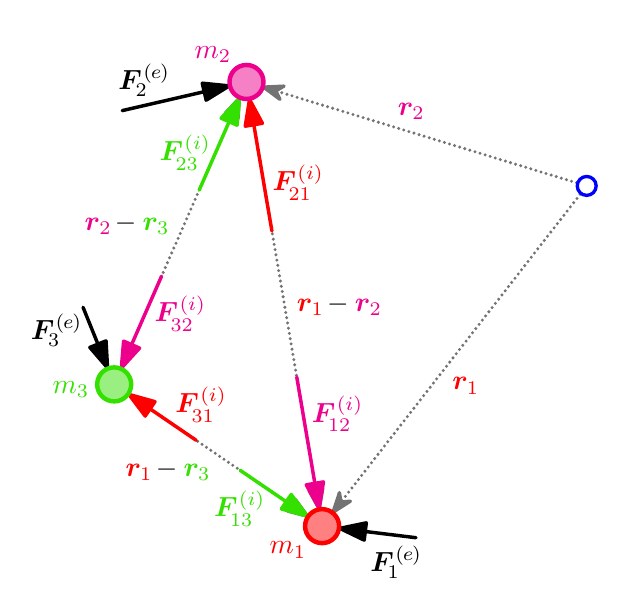
\begin{tikzpicture}[scale=1.2]

% arguments: name, x, y, radius
\newcommand{\setpointmass}[4]{%
\path (#2, #3) node [shape=coordinate] (#1) {} ;
\def\linewidth{1.6pt}
\pgfmathsetmacro\radiusoffset{#4 - \linewidth}
\path (#1) node [line width=1pt, minimum size=#4, circle, inner sep=\radiusoffset, outer sep=0] (#1circle) {} ;
%%\draw [line width=\linewidth, black, fill=black!50] (#1) circle (#4) ;
%%\path (#1circle) node [black, above left, inner sep=6pt, outer sep=0] {#1} ;
}

% arguments: name, radius, color
\newcommand{\drawpointmass}[3]{%
\def\linewidth{1.6pt}
\draw [line width=\linewidth, #3, fill=#3!50] (#1) circle (#2) ;
}

% arguments: name, color, node options, text
\newcommand{\labelpointmass}[4]{%
\path (#1circle) node [#2, #3] {#4} ;
}

% arguments: name of point, name of force, vector length, vector angle in degrees, color
\newcommand{\forceatpoint}[5]{%

\tikzstyle{force line} =
	[line width=1.25pt, line cap=round, -{Triangle[round, length=4.2mm, width=2.7mm]}]

% (from)!length!angle:(to)
\path ($ (#1)!#3!#4:($ (#1) + (0, #3) $) $) node [shape=coordinate] (#1#2force) {} ;

\draw [force line, #5] (#1#2force) -- (#1circle) {} ;
}

% arguments: name of point, name of other point, name of force, force vector length, color
\newcommand{\forcebetweenpoints}[5]{%

\tikzstyle{force line} =
	[line width=1.25pt, line cap=round, -{Triangle[round, length=4.2mm, width=2.7mm]}]

\path ($ (#1)!#4!0:(#2) $) node [shape=coordinate] (#1#3force) {} ;

\draw [force line, #5] (#1#3force) -- (#1circle) {} ;
}

% arguments: name of point, name of force, position, node options, text
\newcommand{\labelforceatpoint}[5]{%
\node at ($ (#1#2force)!#3!(#1) $) [#4] {#5} ;
}

\tikzset{%
radiiline/.style={line cap=round, dash pattern=on 0pt off 1.6\pgflinewidth, -{Stealth[round, length=3.8mm, width=2.7mm]}}%
}

\def\mthirdcolor{green!77!yellow!88!black}

\setpointmass{m1}{35mm}{-28mm}{2mm}
\setpointmass{m2}{27mm}{19mm}{2mm}
\setpointmass{m3}{13mm}{-13mm}{2mm}

\path (63mm, 8mm) node [shape=coordinate] (O) {} ;

% draw position vectors

\draw [radiiline, line width=1.2pt, black!55] (O) -- (m1circle)
	node [red, pos=0.56, below right, inner sep=3pt, outer sep=0] {$\bm{r}_1$} ;

\draw [radiiline, line width=1.2pt, black!55] (O) -- (m2circle)
	node [magenta, pos=0.54, above, inner sep=4.7pt, outer sep=0] {$\bm{r}_2$} ;

\draw [radiiline, line width=1.2pt, black!55] (m2circle) -- (m1circle)
	node [black, pos=0.55, above right, inner sep=3.3pt, outer sep=0] {$\mathcolor{red}{\bm{r}_1} \hspace{-0.25ex} - \mathcolor{magenta}{\bm{r}_2}$} ;

\draw [radiiline, line width=1.2pt, black!55] (m3circle) -- (m2circle)
	node [black, pos=0.47, above left, inner sep=2.6pt, outer sep=0] {$\mathcolor{magenta}{\bm{r}_2} \hspace{-0.25ex} - \mathcolor{\mthirdcolor}{\bm{r}_3}$} ;

\draw [radiiline, line width=1.2pt, black!55] (m3circle) -- (m1circle)
	node [black, pos=0.49, below left, inner sep=2.1pt, outer sep=0] {$\mathcolor{red}{\bm{r}_1} \hspace{-0.25ex} - \mathcolor{\mthirdcolor}{\bm{r}_3}$} ;

% draw force vectors

\forceatpoint{m1}{ext}{10mm}{263}{black}
\labelforceatpoint{m1}{ext}{0.22}{below, outer sep=6.3pt, inner sep=0}{${\bm{F}^{\smthexternal}_{\hspace{-0.15ex}1}}$}

\forceatpoint{m2}{ext}{13.5mm}{103}{black}
\labelforceatpoint{m2}{ext}{0.17}{above, outer sep=3.3pt, inner sep=0}{${\bm{F}^{\smthexternal}_{\hspace{-0.15ex}2}}$}

\forceatpoint{m3}{ext}{8.8mm}{22}{black}
\labelforceatpoint{m3}{ext}{0.34}{left, outer sep=4.7pt, inner sep=0}{${\bm{F}^{\smthexternal}_{\hspace{-0.15ex}3}}$}

\forcebetweenpoints{m1}{m2}{int12}{16mm}{magenta}{-2mm}
\labelforceatpoint{m1}{int12}{0.27}{magenta, right, outer sep=3pt, inner sep=0}{${\bm{F}^{\smthinternal}_{\raisebox{-0.1em}{$\scriptstyle \hspace{-0.25ex}12$}}}$}

\forcebetweenpoints{m2}{m1}{int21}{16mm}{red}{2mm}
\labelforceatpoint{m2}{int21}{0.3}{red, right, outer sep=3pt, inner sep=0}{${\bm{F}^{\smthinternal}_{\raisebox{-0.1em}{$\scriptstyle \hspace{-0.25ex}21$}}}$}

\forcebetweenpoints{m3}{m2}{int32}{12.5mm}{magenta}
\labelforceatpoint{m3}{int32}{0.38}{magenta, right, outer sep=4pt, inner sep=0}{${\bm{F}^{\smthinternal}_{\raisebox{-0.1em}{$\scriptstyle \hspace{-0.25ex}32$}}}$}

\forcebetweenpoints{m2}{m3}{int23}{12.5mm}{\mthirdcolor}
\labelforceatpoint{m2}{int23}{0.63}{\mthirdcolor, below left, outer sep=7.2pt, inner sep=0}{${\bm{F}^{\smthinternal}_{\raisebox{-0.1em}{$\scriptstyle \hspace{-0.25ex}23$}}}$}

\forcebetweenpoints{m1}{m3}{int13}{10.5mm}{\mthirdcolor}
\labelforceatpoint{m1}{int13}{0.37}{\mthirdcolor, below left, outer sep=2.5pt, inner sep=0}{${\bm{F}^{\smthinternal}_{\raisebox{-0.1em}{$\scriptstyle \hspace{-0.25ex}13$}}}$}

\forcebetweenpoints{m3}{m1}{int31}{10.5mm}{red}
\labelforceatpoint{m3}{int31}{0.28}{red, above right, outer sep=0.8pt, inner sep=0}{${\bm{F}^{\smthinternal}_{\raisebox{-0.1em}{$\scriptstyle \hspace{-0.25ex}31$}}}$}

% draw points

\drawpointmass{m1}{1.8mm}{red}
\labelpointmass{m1}{red}{below left, inner sep=5.7pt, outer sep=0}{$m_1$}

\drawpointmass{m2}{1.8mm}{magenta}
\labelpointmass{m2}{magenta}{above left, xshift=1.4pt, inner sep=6.9pt, outer sep=0}{$m_2$}

\drawpointmass{m3}{1.8mm}{\mthirdcolor}
\labelpointmass{m3}{\mthirdcolor}{left, yshift=-2pt, inner sep=9pt, outer sep=0}{$m_3$}

\draw [line width=1.2pt, blue, fill=white] (O) circle (1mm) ;

\end{tikzpicture}

\end{document}
